Nykyisen arkkitehtuurin ongelma ovat useat integroinnin LDAP-palvelimeen. LDAP:in on talletettu jäsenten henkilökohtaista dataa, kuten henkilötunnus, joten tietoturvasyistä siihen halutaan integroida mahdollisimman vähän eri sovelluksia. Tällä hetkellä sovelluksia on vain Sikteeri ja admtool, mutta pidemmän aikavälin tavoitteena on uusien palveluiden (kuten käyttäjien palvelunhallinta) toteuttaminen sekä nykyisen Sikteerin jakaminen pienempiin osapalveluihin palvelusuuntautuneen arkkitehtuurin mukaisesti. Kuvassa \ref{kapsi_uusi} on esitetty tavoiteltu arkkitehtuuri, jossa Sikteerin laskutus- ja jäsenrekisteripalvelut on itsenäisiä web-sovelluksia ja joiden rinnalla on admtool-komentorivityökalu sekä käyttäjien palvelunhallinta. LDAP:n integraatiopisteiden määrä on yksi, sillä LDAP kommunikoi vain keskitetyn tunnistautumispalvelun kanssa, joka taas tarjoaa Kapsi ry:n web-sovelluksille tunnistautumisrajapinnat.

\begin{figure}[ht]
\centering
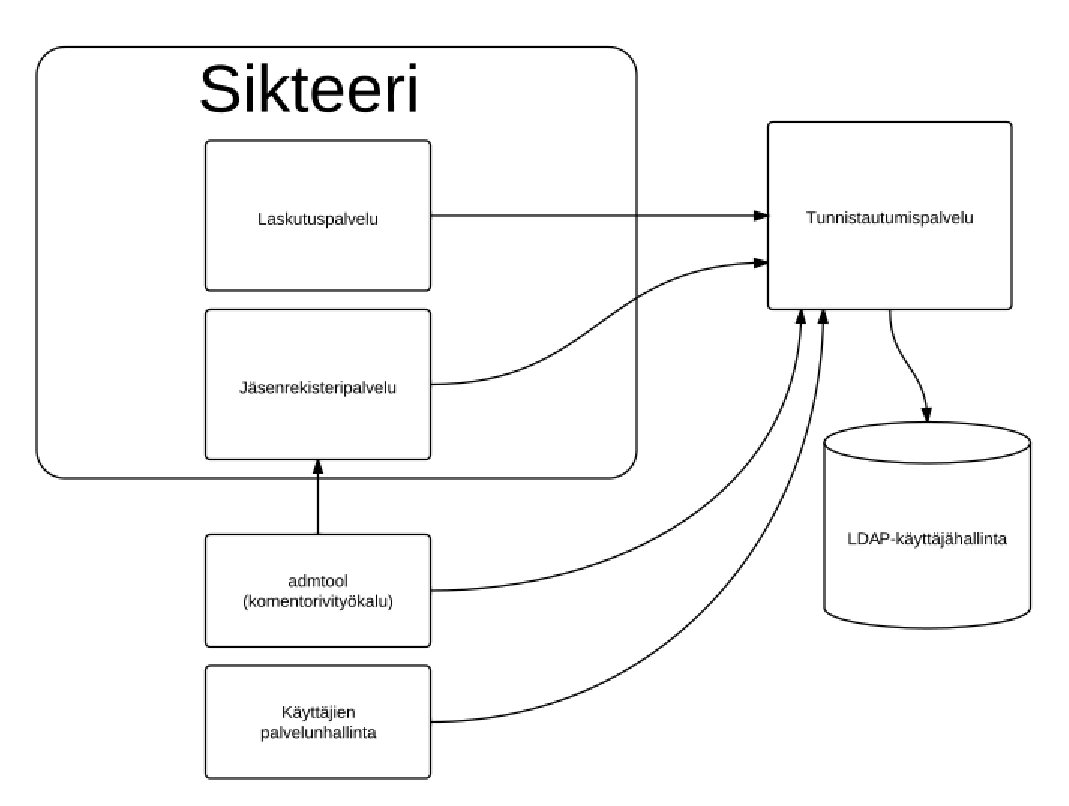
\includegraphics[width=.7\textwidth]{toteutus/kapsi_uusi.eps}
\caption{Palvelusuuntautuneen arkkitehtuurin mukainen kuvaus Kapsin järjestelmästä. Sikteerin palvelut on jaoteltu omiksi komponenteiksi ja järjestelmään on lisätty keskitetty tunnistautumispalvelu.}%
\label{kapsi_uusi}
\end{figure}

Tämän tutkielman kannalta oleellisin osa uudessa arkkitehtuurissa on keskitetyn tunnistautumispalvelun toteuttaminen. Sikteerin nykyinen toteutus ja suunniteltu jatkokehitys asettavat tiettyjä vaatimuksia toteutettavalle tunnistautumispalvelulle. Näitä vaatimuksia sekä muita reunaehtoja käsitellään seuraavassa alaluvussa.

\subsubsection{Vaatimukset ja reunaehdot}
Nykyinen toimintaympäristö, sekä Kapsin omat käytännöt, asettavat vaatimuksia ja reunaehtoja toteutukselle. Enimmäkseen nämä vaatimukset johtuvat käytetystä Python-kielestä ja halusta tukea avointa ohjelmistokehitystä.

Järjestelmän ylläpidon helpottamiseksi uudet komponentit halutaan toteuttaa Pythonilla, koska Sikteeri ja admtool on toteutettu sillä. Toteutuksessa halutaan käyttää mahdollisimman paljon avoimen lähdekoodin alaista koodia, joten tunnistautumispalvelussa käytetystä protokollasta täytyy olla Python-kielellä toteutettu ratkaisu. Toisaalta järjestelmän sisällä ei haluta sulkea muiden ohjelmointikielten tai -kehysten käyttöä pois, joten pelkästään Python-kielinen ratkaisu ei riitä, vaan standardejen täytyy olla avoimia ja käytettävissä myös Javan web-kehyksillä tai esimerkiksi Ruby on Rails -ohjelmointikehyksellä.

Tunnistautumispalvelun täytyy tukea myös komentorivityökaluja, kuten nykyistä admtoolia. Tällöin pelkkä käyttäjäagentti-pohjainen tunnistamismenetelmä ei riitä, vaan tunnistamisen täytyy olla mahdollista ilman selainta.

Käyttäjän tunnistaminen ei riitä yksinään, vaan tunnistautumispalvelun täytyy tukea myös käyttäjään liittyvien parametrien välitystä. Tämä on tärkeää, koska järjestelmässä on eri tasoisia käyttäjiä (hallitus, toimihenkilöt ja ylläpito) ja tunnistautumispalvelua käyttävän sovelluksen täytyy tietää, mihin käyttäjäryhmään tunnistettu käyttäjä kuuluu. Myös muita käyttäjään liittyviä attribuutteja, kuten sähköpostiosoitetta tai puhelinnumeroa, tarvitaan sovelluksissa.

Valitun tunnistautumisprotokollan täytyy olla sellainen, että nykyisten sovellusten muuttaminen käyttämään uutta tunnistautumismekanismia on helppoa. Tämä tarkoittaa, että koodiin täytyy tehdä mahdollisimman vähän muutoksia. Nykyisissä toteutuksissa on käytetty Djangon vakio-tunnistautumismekanismia, joka toimii väliohjelmakerroksessa. Käytettävästä tunnistautumisprotokollasta olisi hyvä olla valmis avoimen lähdekoodin Django-valiohjelmatoteutus jo olemassa.